\documentclass[runningheads]{llncs}
\usepackage[T1]{fontenc}
\usepackage{amsmath,amssymb}
\usepackage{graphicx}
\usepackage{booktabs}
\usepackage{algorithm}
\usepackage[noend]{algpseudocode}
\usepackage{xcolor}
\usepackage{hyperref}
\hypersetup{colorlinks=true,linkcolor=blue!50!black,citecolor=blue!50!black,urlcolor=blue!50!black}

\newcommand{\R}{\mathbb{R}}
\newcommand{\Rec}{\mathcal{R}}
\newcommand{\dom}{\Omega}
\newcommand{\src}{\sigma}
\DeclareMathOperator*{\argmax}{arg\,max}

\begin{document}
\title{Exact Backpropagation through Morphological Reconstruction with Provenance Maps}
\titlerunning{Exact Backpropagation through Morphological Reconstruction}
\author{Anonymous Author(s)}
\authorrunning{Anonymous}
\institute{Anonymous Institution}
\maketitle

\begin{abstract}
Morphological reconstruction underlies the $h$-maxima and $h$-dome transforms, openings by reconstruction, hole filling and many connected operators. Recent works insert it into neural networks by unrolling geodesic dilations until stability and backpropagating through the resulting computational graph. The memory of this approach grows with the number of iterations, i.e.\ with the geodesic diameter of the image, and truncating the loop silently changes the gradient. We observe that reconstruction is a max--min (bottleneck) path function: every output value is a copy of exactly one input value, either from the marker or from the mask. We prove that, for inputs with pairwise distinct values, reconstruction is differentiable and its Jacobian has one-hot rows given by this \emph{provenance}, and that it coincides with the gradient of the fully unrolled loop. We give a parallel algorithm that computes the provenance map alongside the reconstruction with memory independent of the number of iterations; the backward pass is then a single scatter-add. For the $h$-dome transform, the gradient is supported on the domes, the regional maxima and the saddles of the image, which ties learning to the classical notion of dynamics. On GPU, our layer reduces training memory by one to three orders of magnitude and makes reconstruction on large images and long geodesic paths tractable. Training a U-Net end-to-end through an $h$-dome layer for nucleus detection on BBBC039 removes the need for post-hoc tuning of $h$.
\keywords{Morphological reconstruction \and $h$-maxima \and Dynamics \and Morphological neural networks \and Automatic differentiation}
\end{abstract}

%-------------------------------------------------------------------------------
\section{Introduction}
Geodesic reconstruction~\cite{vincent1993,soille2003} is one of the most versatile tools of mathematical morphology. Reconstruction by dilation of a marker $f$ under a mask $g\ge f$ propagates the values of $f$ inside the regional structure of $g$; it underlies the $h$-maxima and $h$-dome transforms, regional extrema, openings and closings by reconstruction, hole filling and, through the dynamics of extrema~\cite{grimaud1992}, the marker selection step of most watershed pipelines~\cite{naylor2019}.

Bringing morphology into deep networks is an active topic~\cite{romerogarcia2026}. For dilations and erosions by a structuring function, the max and min are either smoothed~\cite{masci2013,hermary2022,kirszenberg2021} or differentiated through their subgradients~\cite{franchi2020,blusseau2024,dimitrova2025}. Reconstruction is different: it is the \emph{limit} of a sequence of geodesic dilations whose length is data-dependent. Liu et al.~\cite{liu2024,blusseau2025} introduced geodesic reconstruction layers to count cells with trainable $h$-maxima. Their layer iterates geodesic dilations in a loop until stability, and gradients are obtained by automatic differentiation through the unrolled loop. This raises two problems. (i)~\emph{Memory}: autograd stores every iterate, so memory is $O(NK)$ for $N$ pixels and $K$ iterations, and $K$ is the geodesic diameter of the propagation domain, which can be $\Theta(N)$. (ii)~\emph{Bias}: capping $K$ to save memory gives the exact gradient of a \emph{different} operator, namely $K$ geodesic dilations. In~\cite{blusseau2025} the gradient with respect to the image is stopped and only $h$ is learned; letting gradients reach the image, and hence the network that produces it, is the natural next step.

We show that neither problem is necessary. Our observation is elementary: the reconstruction value at a pixel is a max--min over paths, so it \emph{equals} one input value, which we call its provenance. Our contributions are:
\begin{itemize}
\item a characterisation of the derivative of reconstruction: for inputs with pairwise distinct values it exists, its Jacobian rows are one-hot vectors given by the provenance map, and it equals the derivative of the fully unrolled loop (Sect.~\ref{sec:theory});
\item a geometric reading for the $h$-dome transform: the gradient is supported on domes, regional maxima and saddles, so learning through $h$-domes acts directly on the dynamics of maxima (Prop.~\ref{prop:hdome});
\item a parallel algorithm that computes provenance alongside reconstruction with memory independent of the number of iterations. Its backward pass is one scatter-add, and its static buffers allow the whole iteration to be captured as a CUDA graph (Sect.~\ref{sec:algo});
\item experiments on correctness, gradient bias under truncation, efficiency, and end-to-end nucleus detection through an $h$-dome layer (Sect.~\ref{sec:exp}). Code is available.\footnote{Repository link withheld for review.}
\end{itemize}

\paragraph{Related work.} Our analysis is close in spirit to ultrametric fitting by gradient descent~\cite{chierchia2019}, where the subdominant ultrametric, a min--max path distance, is differentiated by selecting the minimum-spanning-tree edge that realises each value. We transpose this selection principle to grey-level reconstruction on images, where the selection is computed on the fly by a parallel algorithm, and we relate the selected elements to the critical points of the image. Implicit differentiation of fixed points~\cite{bai2019} is another way to avoid unrolling, but reconstruction is a non-smooth fixed point with an explicit combinatorial structure that we exploit directly. Piecewise-affine selection functions~\cite{scholtes2012} and the Bouligand-derivative analysis of morphological layers~\cite{blusseau2024} give the general non-smooth background.

%-------------------------------------------------------------------------------
\section{Reconstruction as a Selection Function}\label{sec:theory}
Let $\dom$ be a finite set of $N$ pixels with a symmetric adjacency ($4$- or $8$-adjacency in 2D), and let $\mathcal N(p)$ be the neighbourhood of $p$, including $p$. For $X\in\R^\dom$, $\delta X(p)=\max_{q\in\mathcal N(p)}X(q)$. Given a marker $f$ and a mask $g$, the geodesic dilation is $\delta_g X=\delta X\wedge g$, and reconstruction by dilation is
\begin{equation}
\Rec_g(f)=\lim_{k\to\infty}X_k,\qquad X_0=f\wedge g,\quad X_{k+1}=\delta_g X_k .
\end{equation}
The sequence is non-decreasing and bounded by $g$ on a finite domain, so it is stationary after $K^\ast(f,g)$ iterations, the \emph{stability index}. We write $z=(f,g)\in\R^{2N}$ for the concatenated inputs and index its entries by $\dom\times\{\mathrm m,\mathrm k\}$ (marker, mask). A path is a sequence $\pi=(p_0,\dots,p_\ell)$ of successively adjacent pixels.

\begin{proposition}[path formula~\cite{vincent1993}]\label{prop:path}
$X_k(p)=\max_{\pi}\min\big(f(p_0),g(p_0),\dots,g(p_\ell)\big)$, where the maximum runs over paths of length $\ell\le k$ ending at $p_\ell=p$. $\Rec_g(f)(p)$ is given by the same formula with no length restriction.
\end{proposition}
\begin{proof}
The claim holds for $k=0$ (trivial path). If it holds for $X_k$, then $X_{k+1}(p)=\min\big(g(p),\max_{q\in\mathcal N(p)}X_k(q)\big)$ is the max over paths of length $\le k$ ending at a neighbour $q$, extended by $p$, of the min of the previous terms and $g(p)$.\qed
\end{proof}

Each $X_k(p)$, and therefore $\Rec_g(f)(p)$, is a \emph{lattice polynomial} $\max_i\min_{j\in S_i}z_j$ in the entries of $z$, and consequently equals one of them. We call any index $\src(p)\in\dom\times\{\mathrm m,\mathrm k\}$ with $\Rec_g(f)(p)=z_{\src(p)}$, realised by a minimiser of an optimal path, a \emph{provenance} of $p$, and the map $\src$ a provenance map.

\begin{proposition}[derivative]\label{prop:deriv}
Let $z$ have pairwise distinct entries. Then $\src(p)$ is unique for every $p$, $\Rec$ is differentiable at $z$, and
\begin{equation}
\frac{\partial\Rec_g(f)(p)}{\partial z_j}=\mathbb 1\big[j=\src(p)\big].\label{eq:jac}
\end{equation}
Consequently, for a loss $L$ with upstream gradient $\bar R=\partial L/\partial\Rec$, the vector--Jacobian product is $\bar z_j=\sum_{p:\,\src(p)=j}\bar R(p)$.
\end{proposition}
\begin{proof}
Uniqueness is immediate since the values are distinct. A lattice polynomial is evaluated by comparisons only, so on the open set $U\ni z$ of vectors whose entries have the same strict order as those of $z$, the term index achieving the max and the entry achieving the min are the same as at $z$. Hence $\Rec_g(f)(p)=z'_{\src(p)}$ for all $z'\in U$, a linear function of $z'$.\qed
\end{proof}

Inputs with ties form a finite union of hyperplanes, a Lebesgue-null set; network outputs are continuous-valued and almost never hit it. $\Rec$ is moreover piecewise linear and $1$-Lipschitz for $\|\cdot\|_\infty$. On ties, our implementation returns a one-hot selection of an entry equal to the output and realised by a propagation path, which is the same convention as autograd applied to max/min.

\begin{proposition}[unrolled autograd]\label{prop:unrolled}
Let $z$ have pairwise distinct entries and $K\ge K^\ast(z)$. The derivative of the $K$-fold unrolled map $z\mapsto X_K$ at $z$ equals \eqref{eq:jac}, whatever tie-breaking rule autograd uses inside the max and min operations. For $K<K^\ast(z)$ it is the derivative of $X_K\ne\Rec_g(f)$.
\end{proposition}
\begin{proof}
By Prop.~\ref{prop:path} and the argument of Prop.~\ref{prop:deriv}, on $U$ we have $X_K(p)=z'_{\src_K(p)}$ for a fixed index $\src_K(p)$. At $z$, $X_K=\Rec_g(f)$ and the entries are distinct, so $\src_K=\src$. Inside the loop, ties only occur between copies of the same entry $z_j$: two iterates that are equal at $z$ select the same index, and both are locally equal to $z'_j$. Any convex split of the gradient between them therefore sums to the same derivative $e_j$, and the chain rule gives \eqref{eq:jac}.\qed
\end{proof}

Proposition~\ref{prop:unrolled} makes the cost of unrolling explicit. To be exact, autograd must store $K^\ast$ iterates. Truncating the loop gives, at every pixel not yet reached by the propagation, a gradient that points to $g(p)$ or $f(p)$ instead of the true source.

\paragraph{The $h$-dome transform and dynamics.} For an image $u$ and $h>0$, the $h$-dome transform is $D_h(u)=u-\Rec_u(u-h)$, and the $h$-maxima are the regional maxima of $\Rec_u(u-h)$. Both arguments of $\Rec$ depend on $u$, so for generic $(u,h)$ Prop.~\ref{prop:deriv} gives
\begin{equation}
\frac{\partial D_h(u)(p)}{\partial u}=e_p-e_{s(p)},\qquad \frac{\partial D_h(u)(p)}{\partial h}=\mathbb 1\big[\src(p)\in\dom\times\{\mathrm m\}\big],\label{eq:hdome}
\end{equation}
where $s(p)\in\dom$ is the pixel of $\src(p)$. The source pixels have a precise meaning:

\begin{proposition}[peaks and saddles]\label{prop:hdome}
Let $u$ have pairwise distinct values, as well as the values of $u-h$ and $u$ together, and let $p$ belong to a dome, i.e.\ $D_h(u)(p)>0$. If the provenance of $p$ lies in the marker, $s(p)$ is a regional maximum of $u$. If it lies in the mask, $s(p)$ is a \emph{saddle} of $u$: it has two neighbours that lie in distinct connected components of the upper level set $\{u>u(s(p))\}$.
\end{proposition}
\begin{proof}
\emph{Marker.} Let $\pi$ be an optimal path from $q=s(p)$ with value $u(q)-h$. If $q$ had a neighbour $q'$ with $u(q')>u(q)$, prefixing $\pi$ with $q'$ would give a path with value $\min(u(q')-h,u(q'),\min_\pi u)$. This is $\ge u(q)-h$, and it is $>u(q)-h$ unless another entry equals $u(q)-h$, which genericity excludes. This contradicts optimality, so $q$ is a regional maximum. \emph{Mask.} Then $r=s(p)$ is the unique minimiser of an optimal path $\pi$ from some $q$ to $p$, and $u(r)=\Rec(p)<u(p)$ because $p$ is in a dome, so $r\ne p$. If $r=q$, then $u(q)-h<u(q)$ would be a smaller term, a contradiction; so $r$ has a predecessor $a$ and a successor $b$ on $\pi$. Assume $a$ and $b$ are connected in $\{u>u(r)\}$. Replacing the sub-path $a\to r\to b$ by such a connection gives a path whose terms all exceed $u(r)$, because $u(q)-h>u(r)$ by uniqueness of the minimiser. Then $\Rec(p)>u(r)$, a contradiction.\qed
\end{proof}

Hence the gradient of any loss on $D_h(u)$ is supported on the domes and on the critical points of $u$ that define the \emph{dynamics} of its maxima~\cite{grimaud1992}: the peaks, whose dynamic exceeds $h$, and the saddles at which lower domes are cut. A loss can therefore raise or lower a peak, or deepen the pass between two touching objects, through the exact pixel that controls it (Fig.~\ref{fig:illus}). This is precisely what end-to-end learning of object detection by $h$-maxima requires.

\begin{figure}[t]
\centering
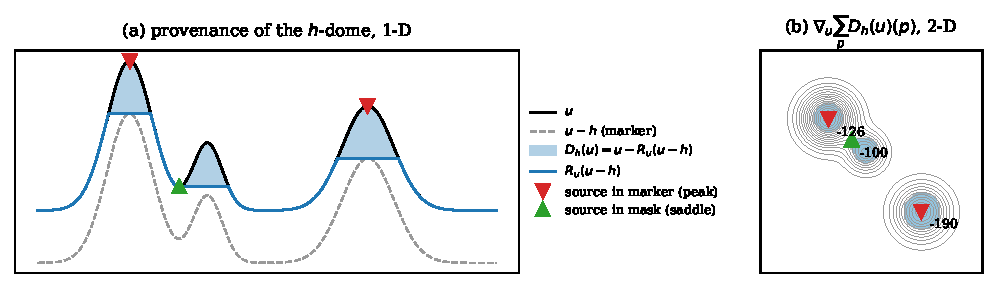
\includegraphics[width=\textwidth]{figures/illustration.pdf}
\caption{(a) Provenance of the $h$-dome on a 1-D signal: dome values are copied from a peak (marker, \textcolor{red!70!black}{$\blacktriangledown$}) or from a saddle (mask, \textcolor{green!50!black}{$\blacktriangle$}). (b) Gradient of $\sum_p D_h(u)(p)$ on a 2-D image: $+1$ on dome pixels (blue) and a single negative mass on each source pixel (counts printed), as predicted by \eqref{eq:hdome} and Prop.~\ref{prop:hdome}.}\label{fig:illus}
\end{figure}

%-------------------------------------------------------------------------------
\section{Computing Provenance in Parallel}\label{sec:algo}
Algorithm~\ref{alg:prov} augments the parallel geodesic-dilation scheme with a provenance map $\src_k$, stored as an integer image of flat indices in $[0,2N)$. It keeps the invariant
\begin{equation}
X_k(p)=z_{\src_k(p)}\quad\text{and}\quad X_k=\delta_g^k(f\wedge g)\qquad\text{for all }k,\label{eq:inv}
\end{equation}
because each assignment of a value copies the provenance of that value. A pixel is updated only on a \emph{strict} increase, so ties never overwrite a valid provenance. The stability test is performed every $c$ iterations ($c=16$), and the extra iterations are harmless because $\Rec$ is idempotent.

\begin{algorithm}[t]
\caption{Reconstruction by dilation with provenance (all operations are pixel-parallel)}\label{alg:prov}
\begin{algorithmic}[1]
\Require marker $f$, mask $g$, neighbourhood offsets $\mathcal O\ni 0$
\State $X\gets f\wedge g$; \quad $\src(p)\gets p$ if $f(p)\le g(p)$ else $p+N$
\Repeat
  \State $(B,a)\gets \max/\argmax_{o\in\mathcal O} X(\cdot+o)$ \Comment{one stacked reduction; $-\infty$ outside $\dom$}
  \State $\beta(p)\gets\src(p+a(p))$ \Comment{gather the provenance of the winning neighbour}
  \State $C\gets B\wedge g$;\quad $\gamma(p)\gets p+N$ if $B(p)>g(p)$ else $\beta(p)$
  \State where $C>X$: \ $X\gets C$,\ $\src\gets\gamma$
\Until{$X$ is unchanged}
\State \Return $X,\src$ \Comment{backward: $\bar z\gets 0$;\ \ $\bar z[\src(p)]\mathrel{+}=\bar R(p)$ for all $p$}
\end{algorithmic}
\end{algorithm}

\paragraph{Complexity.} Each iteration costs $O(|\mathcal O|N)$ operations, like an unrolled geodesic dilation, but no computational graph is stored. Memory is $O(|\mathcal O|N)$ for the stacked reduction plus $O(N)$ for $X$ and $\src$, independent of $K^\ast$; the backward pass is one $O(N)$ scatter-add. Unrolled autograd needs $\Theta(K^\ast N)$ memory, with $K^\ast$ up to $\Theta(N)$ for winding propagation domains. Because all buffers are allocated once, a chunk of $c$ iterations can be recorded as a CUDA graph and replayed, which removes the kernel-launch overhead that dominates parallel reconstruction on small and medium images. The dual reconstruction by erosion is obtained as $-\Rec_{-g}(-f)$, and the same code handles batches, channels and 3-D volumes. Finally, any sequential reconstruction algorithm (hybrid~\cite{vincent1993}, downhill filter~\cite{robinson2004}, union-find~\cite{najman2006}) can be augmented in the same way: whenever it assigns $X(q)\gets X(p)\wedge g(q)$, it also sets $\src(q)\gets\src(p)$ or $q+N$.

%-------------------------------------------------------------------------------
\section{Experiments}\label{sec:exp}
All experiments use PyTorch on a laptop RTX~4060 GPU (8\,GB) and $8$-adjacency unless stated otherwise.

\paragraph{Correctness.} Our forward pass matches \texttt{skimage.morphology.reconstruction} (dilation and erosion, 2-D and 3-D, both adjacencies) to machine precision. On float64 random inputs, the gradients with respect to both marker and mask coincide with those of the fully unrolled loop to $10^{-12}$ (Prop.~\ref{prop:unrolled}), and they pass finite-difference \texttt{gradcheck} for $\Rec$ and for $D_h$ with respect to both $u$ and $h$. These checks are part of the released test suite.

\begin{figure}[t]
\centering
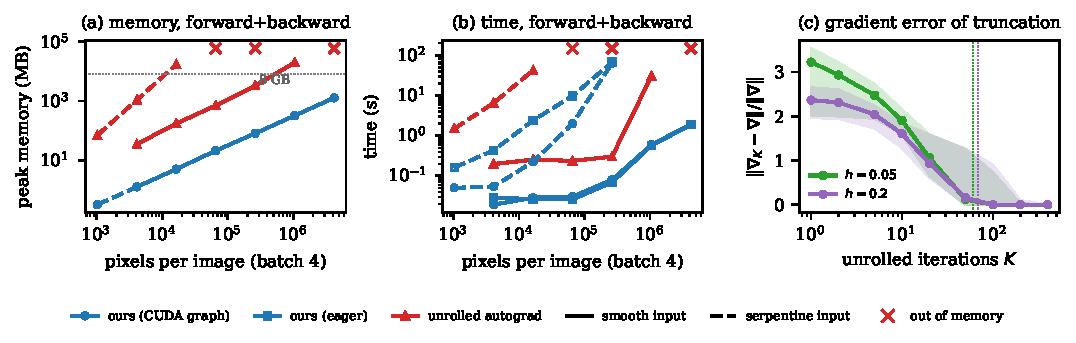
\includegraphics[width=\textwidth]{figures/bench.pdf}
\caption{(a,b) Peak GPU memory and time of one forward and backward pass through $\Rec$ (batch of 4 float32 images), for smooth random images ($K^\ast\le 59$) and serpentine masks with a single seed ($K^\ast\approx N/2$). The unrolled point at $1024^2$ (19.7\,GB) ran only because the driver spilled to host memory. (c) Relative error of the gradient of $\sum_p w(p)D_h(u)(p)$ ($w$ Gaussian) obtained by autograd through $K$ unrolled iterations, on 20 smoothed $256^2$ BBBC039 crops (median and 10--90\% band). Dotted lines: median stability index $K^\ast$.}\label{fig:bench}
\end{figure}

\paragraph{Efficiency.} Figure~\ref{fig:bench}(a,b) compares our layer with the unrolled loop with autograd, the approach of~\cite{liu2024,blusseau2025}, on two families of inputs. \emph{Smooth} images reach stability in $20$--$60$ iterations. \emph{Serpentine} masks, a single 2-pixel-wide corridor folded over the image with a seed at one end, have $K^\ast\approx N/2$. On smooth inputs, the unrolled graph needs $41\times$ more memory than our layer at $512^2$ (3.3\,GB vs.\ 81\,MB) and $62\times$ more at $1024^2$, where it exceeds the 8\,GB of the device. At $2048^2$ it fails, while ours needs 1.3\,GB. On serpentines, the memory of the unrolled loop grows as $NK^\ast=\Theta(N^2)$: 17.3\,GB already at $128^2$, against 5\,MB for ours, and it fails from $256^2$ on. Our memory is the same for both families, as predicted. Our backward pass takes less than 5\,ms in every case. Thanks to CUDA-graph replay, our forward iterations are also several times cheaper than unrolled ones: a full forward and backward pass is $8\times$ faster at $256^2$ on smooth inputs and $190\times$ faster on the $128^2$ serpentine. Without graph capture (eager mode) the forward pass is launch-bound on small images and comparable to an unrolled forward pass, but the memory advantage remains.

\paragraph{Bias of truncated unrolling.} Figure~\ref{fig:bench}(c) measures what is lost when the loop is capped to save memory. On nucleus images, $K^\ast$ is 60--70 iterations for $256^2$ crops. With $K=20$ the relative gradient error is about $100\%$ (cosine similarity $0.63$--$0.69$); with $K=50$ it is still $12$--$16\%$. Once $K\ge K^\ast$ the error drops to float32 round-off ($<10^{-6}$), as stated by Prop.~\ref{prop:unrolled}. Since $K^\ast$ depends on the image and on the current network output, no fixed cap is safe, whereas our layer is always exact.

%%DETECTION%%

%-------------------------------------------------------------------------------
\section{Conclusion}
Morphological reconstruction is differentiable almost everywhere, with a Jacobian given by provenance: each output pixel copies one input entry. Computing this provenance alongside the reconstruction gives exact gradients with memory independent of the number of propagation steps, equal to those of the fully unrolled loop and obtained at a fraction of its cost. For $h$-domes the gradient lives on peaks and saddles, so training through the layer acts on the dynamics of the predicted map. The same principle extends to openings and closings by reconstruction, levelings and other operators built from reconstruction. Natural next steps are learnable markers for connected filters and extensions to component-tree attributes.

\bibliographystyle{splncs04}
\bibliography{refs}
\end{document}
